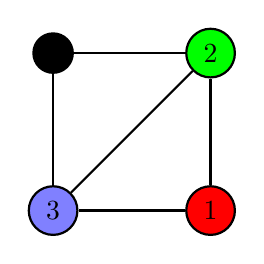
\begin{tikzpicture}[
	% Define the style for the nodes
	every node/.style={circle, draw, thick, minimum size=5mm}
	]
	
	% --- VERTICES ---
	% Format: \node (internal_name) at (x,y) [fill=color] {number};
	
	\node (v1) at (0, 2) [fill=black]  {};
	\node (v2) at (2, 2) [fill=green] {2};
	\node (v3) at (0, 0) [fill=blue!50]{3};
	\node (v4) at (2, 0) [fill=red]{1};
	
	% --- EDGES ---
	% In a K4, there are 6 possible edges. 
	% We omit one (e.g., the diagonal between v1 and v4).
	
	\draw[thick] (v1) -- (v2); % Top edge
	\draw[thick] (v2) -- (v4); % Right edge
	\draw[thick] (v4) -- (v3); % Bottom edge
	\draw[thick] (v3) -- (v1); % Left edge
	\draw[thick] (v2) -- (v3); % Diagonal 1
	
	% Note: The edge (v1) -- (v4) is omitted to make it non-K4.
	
\end{tikzpicture}